% Elsevier journal article, generated by html2tex (elsarticle template).
% Class: elsarticle (CTAN / vendored by MiKTeX). [3p,twocolumn] gives the
% final two-column journal look; switch to [preprint,review,12pt] for a
% double-spaced single-column first-submission manuscript.
\documentclass[3p,twocolumn]{elsarticle}
\usepackage[T1]{fontenc}
% Scalable Times fonts (the Elsevier journal look). Required: microtype's
% font expansion (loaded via the compat preamble) errors on elsarticle's
% default bitmap CM fonts ("auto expansion is only possible with scalable
% fonts"); newtx text+math are fully scalable.
\usepackage{newtxtext}
\usepackage{hyperref}
\usepackage{etoolbox}

% Shared html2tex compatibility preamble (tables, floats, graphics,
% verbatim, pandoc helper macros, numeric citations).
\input{html2tex_compat.tex}
% newtxmath must load AFTER amssymb (pulled in by the compat preamble):
% amssymb-after-newtxmath dies with "\Bbbk already defined".
\usepackage{newtxmath}
\usepackage{xurl}

% ---------------------------------------------------------------------------
% Column-fill strategy — the FOUR settings below are coupled; changing any
% one in isolation reintroduces a visible defect somewhere else. Written
% together because they were learned together by a full render-and-measure
% pass over a 20-page 2-col paper.
%
% (1) \flushbottom: columns stretch to text-area bottom. Alone with rigid
%     \parskip this leaves visible whitespace at the right-column bottom
%     whenever a \section/\subsection is immediately followed by a full-width
%     [t] table*/figure* — LaTeX cannot split the heading from its float and
%     cannot bottom-place a full-width float in 2-col, so the whole chunk
%     kicks to the next page, leaving the current column short.
% (2) \parskip = 0pt plus 1pt: tiny per-paragraph stretch budget. Invisible
%     individually (~1pt across a 12pt paragraph baseline); cumulative
%     ~30pt/page across the ~30 paragraphs of a body page. This is the pool
%     that (1) draws from to fill columns uniformly.
% (3) Rigid \intextsep / \textfloatsep / \floatsep (no plus/minus glue): forces
%     stretch to distribute across parskips only, NEVER as inflated space
%     around a figure/table. Without this, (1) puts most slack into the
%     larger \textfloatsep and produces visible bands around figures.
% (4) Tightened \section (12pt/6pt, was 18pt/9pt) and \subsection (8pt/2pt,
%     was 12pt/3pt) skips: saves ~1 line of vertical budget per heading, so
%     a heading + its first paragraph fits into a shorter column tail. This
%     directly reduces the frequency of case (1) — many section-heading
%     pages that used to kick can now hold the heading in the current
%     column.
%
% Verify: PyMuPDF column-fill audit (max y1 per half-column, footer
% excluded); target L-R diff < 20pt on every non-final page.
% ---------------------------------------------------------------------------
\flushbottom
\AtBeginDocument{\flushbottom}
\setlength{\parskip}{0pt plus 1pt}
\AtBeginDocument{\setlength{\parskip}{0pt plus 1pt}}
\makeatletter
\renewcommand\section{\@startsection{section}{1}{\z@}%
           {12\p@ \@plus 4\p@ \@minus 4\p@}%
           {6\p@ \@plus 4\p@ \@minus 3\p@}%
           {\normalsize\bfseries\boldmath}}
\renewcommand\subsection{\@startsection{subsection}{2}{\z@}%
           {8\p@ \@plus 4\p@ \@minus 4\p@}%
           {2\p@ \@plus 4\p@ \@minus 3\p@}%
           {\normalfont\normalsize\itshape}}
\makeatother
\setlength{\intextsep}{8pt}
\setlength{\textfloatsep}{8pt}
\setlength{\floatsep}{8pt}

% Float-only pages (a lone full-width table*/figure* on a page with no body
% text before it, e.g. a licensing table at the very end of the paper)
% otherwise render with the float vertically centered. Move the elastic glue
% to \@fpbot / \@dblfpbot so floats sit at the page TOP. Full-width
% (table*/figure*) floats use the \@dblfp* skips; single-column ones use
% \@fp*; set both so any float-only page renders the same way.
\makeatletter
\setlength{\@fptop}{0pt}
\setlength{\@fpsep}{8pt plus 0pt}
\setlength{\@fpbot}{0pt plus 1fil}
\setlength{\@dblfptop}{0pt}
\setlength{\@dblfpsep}{8pt plus 0pt}
\setlength{\@dblfpbot}{0pt plus 1fil}
\makeatother

% Reduce elsarticle 3p top-of-title white margin. The default \pprintMaketitle
% starts with \clearpage, then \printFirstPageNotes and generous vskips before
% the \title emission, placing the title well below the top of page 1. Patch
% the emitter to insert a negative vspace right after its \clearpage, so the
% title sits close to the top of the first page. -2.2cm is calibrated for
% [3p,twocolumn]; adjust if a different documentclass option is chosen.
\makeatletter
\patchcmd{\pprintMaketitle}{\clearpage}{\clearpage\vspace*{-2.2cm}}{}{}
\makeatother

\journal{Neurocomputing}

\begin{document}
\begin{frontmatter}
\title{\vspace*{-2\baselineskip}Anomaly Detector Model Selection by Normal Manifold Separability}

% pack_tmlr_bundle.py fills anonymous placeholders; replace with the real
% elsarticle author block (\author[label]{...} + \affiliation) for submission.
\author[hit]{Alexander Apartsin}
\author[afeka]{Yehudit Aperstein\corref{cor1}}
\ead{apersteiny@afeka.ac.il}
\cortext[cor1]{Corresponding author}
\address[hit]{School of Computer Science, Faculty of Sciences, Holon Institute of Technology (HIT), Holon, Israel}
\address[afeka]{Intelligent Systems, Afeka Academic College of Engineering, Tel-Aviv, Israel}

\begin{abstract}
Choosing an anomaly detector for a new dataset is a chicken-and-egg problem: comparing detectors by held-out ROC-AUC requires labeled anomalies, which unsupervised deployments lack. NoMaS ranks a panel of detectors from the unlabeled data alone: cluster the data, hold out a few clusters as stand-in anomalies, fit each detector on the rest, and score how well it flags the held-out clusters, its held-out-cluster separability. Averaged over many held-out clusters, this separability is a label-free estimate of how well a detector has resolved the normal manifold, the competence it needs to separate true anomalies from normal. We evaluate a selector by \emph{regret}, the AUC gap between the best available detector and the one it picks.

We develop NoMaS on a benchmark of 69 datasets spanning tabular, image, text, and time-series modalities, where a label-free self-calibration cuts regret 78 to 93\% below a random pick, within 0.01 AUC of a labels-based oracle. The signal comes from the geometry of normal data alone: regret is unchanged at 0\% contamination, so NoMaS needs no anomalies in its input to find the detector that will catch them. Against the harder bar of committing to one detector, it beats the Isolation Forest default and matches the best fixed detector without knowing in advance which one it is.

To test generalization, we freeze the method and run it, with no further tuning, on 187 previously-unseen tabular datasets from OddBench. There it attains the lowest regret of any label-free strategy and the most robust skill across benchmarks; because the best fixed detector changes from one benchmark to the next, no advance choice is safe, and NoMaS tracks the winner on its own. One limit remains, datasets whose best detector is global rather than local, which a marginal-tail variant partly closes. We release the code, benchmark, and per-dataset results.
\end{abstract}

\end{frontmatter}

\section{Introduction}\label{1-introduction}

Deploying an anomaly detector on a new dataset without labeled anomalies is common in fraud, industrial monitoring, health, and cybersecurity. The best detector for a given problem is not known in advance and varies widely across datasets. Isolation Forest wins on some datasets, LOF on others, ECOD on yet others. Without labels, the practitioner picks by prior, by convenience, or by expensive human review. Model-selection heuristics for the unsupervised case exist (mass-volume and excess-mass curves \cite{ref1}, IREOS \cite{ref2}, MetaOD \cite{ref3}, internal consensus scores \cite{ref4}) but none has become a standard bar the way ROC-AUC has for the labeled case, and their reported gains over naive baselines are modest.

We ask a simpler question: \emph{if we cluster the unlabeled data and treat a small cluster as if it were an anomaly cluster, does the ranking of detectors on this pseudo-anomaly task predict the ranking on real anomalies?} The intuition runs through the detector\textquotesingle s competence. Every anomaly detector is at heart a model of where the normal data lies, and it flags whatever falls outside that model, so a detector is only as good as its grasp of the normal geometry. A detector that has genuinely captured that geometry should recognize any coherent group of points that sits apart from the bulk, including a held-out cluster we designate as a stand-in anomaly. How well it separates that held-out cluster from the rest of the normal data is therefore a readout of how well it has modeled normal structure, the same competence it needs to separate true anomalies from normal. We can then rank detectors by their average pseudo-AUC across many cluster-holdout draws, without ever seeing a label. The reading is faithful to the degree that real anomalies resemble held-out clusters, compact and locally distinct, which is where the method works and, where they do not, where it meets its ceiling.

Our contributions:

\begin{enumerate}
\tightlist
\item
  \textbf{NoMaS}, an unsupervised ranking procedure for anomaly detectors. Cluster once, hold out subsets of clusters as pseudo-anomalies, fit each detector on the complement, aggregate pseudo-AUC across draws.
\item
  A \textbf{regret-based evaluation} of unsupervised detector selection that is threshold-free and stable, avoiding the boundary artifacts of thresholded rank-correlation, and an \textbf{empirical validation} on 69 datasets across four modalities (tabular, image, text, time-series) with 9 canonical PyOD detectors and five seeds. NoMaS cuts selection regret versus random by 73-90\% on all four. The natural consensus baseline scores Spearman $\rho$ = -0.15, worse than random.
\item
  An \textbf{unsupervised auto-calibration} that recovers near-oracle regret on every modality: run a bank of pseudo-anomaly regimes and weight each by its cross-detector pseudo-AUC variance, a label-free measure of how informative the regime is. This weighting reaches 78-93\% below random on all four modalities and cuts regret on the two embedding modalities a further 2-4$\times$ (text from 0.022 to 0.006), because it automatically up-weights a locally-embedded ("hard") regime that exercises the local-density structure embedding detectors need.
\item
  \textbf{A selector that is trustworthy on two axes practitioners care about.} The ranking signal comes from normal-data geometry alone: regret is flat as real anomalies are added to the unlabeled input and unchanged at 0\% contamination (pure normals). And against the demanding baseline of a single fixed detector, NoMaS has the lowest mean regret of any label-free strategy, beating the Isolation Forest default (paired p \textless{} 0.05 on image, text, and tabular; p \textless{} 0.001 on the two embedding modalities) and matching the best fixed detector without knowing which one it is, both in-distribution and on 187 previously-unseen OddBench datasets.
\item
  \textbf{Ablations, panel robustness, and stability} analyses: the hand-designed composite "anomaly-likeness" selector we expected to help was the worst of three; leave-one-detector-out never materially changes the ranking; and calibrated regret is stable across seeds (std $\leq$ 0.002).
\end{enumerate}

\section{Related work}\label{2-related-work}

\textbf{Anomaly detectors and benchmarks.} Established detectors span the standard families: isolation-based (Isolation Forest \cite{ref8}), density-based (LOF \cite{ref9}), boundary-based (one-class SVM \cite{ref10}), distribution-based (COPOD \cite{ref11}, ECOD \cite{ref12}), projection-based (LODA \cite{ref13}, PCA), and deep one-class methods (DeepSVDD \cite{ref14}). Comprehensive surveys \cite{ref15} and empirical studies \cite{ref16} document that no single detector dominates across datasets, which is exactly what makes per-dataset selection necessary. Standardized benchmarks, ODDS-derived collections and their consolidation in ADBench \cite{ref5}, and the PyOD toolbox \cite{ref6} make large-scale comparison feasible; we build directly on both.

\textbf{Unsupervised model and hyperparameter selection.} The central difficulty is choosing among detectors or configurations without labels. Internal metrics score a single detector from properties of its own output: excess-mass and mass-volume curves \cite{ref1}, and the internal relative-evaluation score IREOS \cite{ref2}. These are detector-anchored and do not define a common task on which two detectors are directly comparable. Meta-learning approaches such as MetaOD \cite{ref3} regress from dataset meta-features to expected performance, but require a labeled meta-training corpus and generalize only within its coverage. A recent review \cite{ref17} evaluates a broad set of internal strategies and finds that none is reliably better than naive baselines across benchmarks, motivating fundamentally different signals. NoMaS instead constructs a common pseudo-labeled task per dataset and lets ROC-AUC rank the detectors, needing neither labels nor meta-training.

\textbf{Consensus and outlier ensembles.} Averaging or combining detector scores yields a consensus outlier score used both as an ensemble output and, implicitly, as a selection signal that favors detectors agreeing with the majority \cite{ref4, ref18}. Our experiments show consensus fails as a ranking signal on ADBench ($\rho$ = -0.15): the detectors most correlated with the panel mean are not those most correct on real anomalies. NoMaS does not assume agreement implies correctness; it measures each detector against an externally constructed pseudo-labeled task.

\textbf{Pseudo-labels and self-supervised anomaly detection.} Synthetic-anomaly injection is standard for turning unsupervised detection into a discriminative problem, and its effectiveness depends heavily on how realistic the injected anomalies are \cite{ref7}. Self-supervised methods create surrogate tasks, geometric-transformation prediction \cite{ref19} or learned classification pretexts \cite{ref20}, whose auxiliary loss serves as an anomaly score. All of these use pseudo-labels to \emph{train} a single detector. NoMaS uses pseudo-labels for the different purpose of \emph{ranking} a panel: the pseudo-anomalies (held-out clusters) need not resemble real anomalies well enough to train a detector, only well enough to order detectors by difficulty.

\section{Method}\label{3-method}

A detector that understands normal data well enough to tell its own sub-structure apart should, for the same reason, tell normal from anomalous; we measure the first to predict the second.

Let \(X \in \mathbb{R}^{n \times d}\) be an unlabeled tabular dataset and let \(\mathcal{D} = \{D_1, \dots, D_L\}\) be a panel of anomaly detectors. Each detector produces a decision function \(s_D: \mathbb{R}^d \to \mathbb{R}\) where higher values mean more anomalous. Our goal is a per-dataset ranking \(\pi_X: \mathcal{D} \to \{1, \dots, L\}\) that approximates the ranking \(\pi_X^*\) induced by ROC-AUC on real anomaly labels.

\textbf{Embedding and clustering.} Standardize \(X\) and apply PCA to 16 dimensions (or keep \(d\) if \(d \le 16\)). Cluster the embedding with MiniBatchKMeans at \(K\) clusters, obtaining assignments \(\ell : \{1, \dots, n\} \to \{1, \dots, K\}\).

\textbf{Cluster subset sampling.} Rank clusters by size ascending and let the candidate pool \(\mathcal{C}\) be the smallest half. For each of \(M = 20\) draws, sample from \(\mathcal{C}\) without replacement until the union has size \(\ge \max(20, 0.05 n)\). The union \(S_j\) is the pseudo-anomaly set for draw \(j\). From the complement, uniformly sample 20\% as the pseudo-normal fold \(N_j\); the remainder is the training set \(T_j\).

\textbf{Held-out-cluster separability.} For each detector \(D\) and draw \(j\), fit \(D\) on \(T_j\), score both \(S_j\) and \(N_j\), and compute the pseudo-AUC \(A_{D,j} = \mathrm{AUC}(\mathbf{1}_{S_j}, s_D)\) with \(S_j\) labeled 1 and \(N_j\) labeled 0. This pseudo-AUC is the detector\textquotesingle s held-out-cluster separability: how well its scores pull the excised cluster \(S_j\) apart from the retained normals \(N_j\). If \(D\) fails on \(T_j\), or emits a non-finite or constant score vector, set \(A_{D,j}\) to missing.

\textbf{Aggregation and ranking.} Within one regime, the aggregation is \(\bar A_D = \operatorname{mean}_j A_{D,j}\) over non-missing \(j\), our estimate of detector \(D\)\textquotesingle s normal-manifold separability, and detectors are ranked by \(\bar A_D\) descending. Borda over per-draw ranks and variance-weighted mean perform within $\pm$0.02 $\rho$ of the mean.

\textbf{Auto-calibration over a regime bank.} A single pseudo-anomaly regime (one cluster-selection rule and one \(K\)) can be blind to the structure that separates the best detector from its near-twin. This is most visible on text: held-out compact clusters are separated equally well by global-distance (KNN) and local-density (LOF) detectors, so the regime fails to prefer the LOF that wins on real anomalies. We therefore run a bank of regimes, cluster-selection $\in$ \{smallest, random, hard\} $\times$ \(K\) $\in$ \{30, 50\}, where \emph{hard} holds out clusters embedded among others (small distance to neighboring centroids), which are locally sparse rather than globally isolated. For each regime \(r\) we compute the per-detector mean pseudo-AUC and a weight \(w_r = \operatorname{Var}_D \bar A_{D}^{(r)}\): the variance of pseudo-AUC across detectors, which is large exactly when the regime discriminates the detectors and near zero when it cannot. The final ranking is the \(w_r\)-weighted average of the per-regime detector ranks. The weight uses only pseudo-AUC and never a label; it automatically up-weights whichever regime is informative for the dataset at hand.

\section{Experimental setup}\label{4-experimental-setup}

\textbf{Datasets.} Our primary benchmark is the 35 ADBench Classical \texttt{.npz} files from \cite{ref5}; after a size filter \(200 \le n \le 50{,}000\), 26 datasets remain, spanning anomaly rates from 1.2\% to 39.9\%, dimensions from 5 to 400, and problem domains from health to spam classification. We additionally validate on a second, independently-preprocessed tabular benchmark, DAMI \cite{ref16} (10 datasets after the same size filter and an anomaly-rate filter \(\le 35\%\)), which shares some UCI sources with ADBench but applies the Campos et al. normalization and de-duplication protocol, so it tests robustness to preprocessing rather than to disjoint data. For a frozen external test (Section 5.5) we additionally use OddBench \cite{ref22}, a public collection of 790 tabular anomaly-detection datasets with real-world semantic anomalies (MacrOData-CMU, \href{https://huggingface.co/datasets/MacrOData-CMU/OddBench}{huggingface.co/datasets/MacrOData-CMU/OddBench}); none of it was touched while developing the method, and we hash-sample the evaluation subset by dataset name rather than choosing it by performance. Labels are used only to compute the ground-truth ranking \(\pi_X^*\); NoMaS never sees them.

\textbf{Detectors.} We use nine canonical PyOD detectors \cite{ref6} with fixed default hyperparameters: IForest, LOF, KNN, ECOD, COPOD, HBOS, PCA, CBLOF, LODA (OCSVM is dropped after a repeatable libsvm C-level crash under multi-worker parallelism; panel-robustness in Section 5.3 shows this removal does not materially change the ranking). We separately verify the results with two deep detectors added, AutoEncoder and DeepSVDD \cite{ref14} (an 11-detector panel), in Section 5.4.

\textbf{Ground truth.} For each dataset, we split the normal points 80/20; fit each detector on the 80\% normal training fold; evaluate ROC-AUC on the union of the 20\% normal test fold and all real anomalies. The ordering by ROC-AUC gives \(\pi_X^*\).

\textbf{Primary metric: regret.} A detector selector exists to pick a good detector, so we measure it by what the user loses from its choice. Let \(\hat D\) be the detector NoMaS ranks first and \(\mathrm{AUC}^*(D)\) the true ROC-AUC of detector \(D\). The top-1 regret on a dataset is
\[\mathrm{regret@1} = \max_{D} \mathrm{AUC}^*(D) - \mathrm{AUC}^*(\hat D),\]
and regret@3 uses the best of NoMaS\textquotesingle s top three picks. Regret is \textbf{threshold-free} and \textbf{self-neutralizing}: on a dataset where all detectors tie, any pick has regret $\approx$ 0, so ill-posed datasets neither help nor hurt the aggregate and need no filtering. It is also \textbf{decision-relevant}: 0.02 regret means the chosen detector is within 2 AUC points of the best available. We report mean regret across a modality\textquotesingle s datasets, and the standard deviation across five seeds as the stability measure. As a reference, a random-pick selector has regret \(\max_D \mathrm{AUC}^*(D) - \operatorname{mean}_D \mathrm{AUC}^*(D)\).

\textbf{Relative companion: skill.} Absolute regret does not say whether a given loss is large for that dataset. We therefore also report a skill score, \(\mathrm{skill} = 1 - \mathrm{regret@1} / \mathrm{regret}_{\text{random}}\), the fraction of the achievable improvement over a blind pick that the selector captures. It is 1 when the best detector is chosen, 0 when the pick is no better than the panel average, and negative when worse than random; it is undefined and omitted when a dataset is tied (\(\mathrm{regret}_{\text{random}} \approx 0\)). To summarize a benchmark in one number we pool across datasets: \(S = 1 - \sum_i \mathrm{regret}_i / \sum_i \mathrm{regret}_{\text{random},i}\), a Murphy-style skill score whose reference policy is the uniform-random pick and whose perfect score is the oracle, an \(R^2\)-analogue for selection. Pooling weights each dataset by how much the choice mattered, so trivially-tied datasets contribute negligibly to both sums rather than destabilizing a mean of ratios.

\textbf{Secondary metric: rank correlation.} For continuity with prior work we also report Spearman $\rho$ between \(\pi_X\) and \(\pi_X^*\), and top-1 / top-3 hit rates. Because $\rho$ is undefined when \(\pi_X^*\) is tied, we compute it on the subset of datasets whose true-AUC spread (max minus min across detectors) is at least 0.10. This threshold is the source of the instability regret avoids: datasets near the boundary cross it under small numerical perturbations, so the thresholded-$\rho$ mean can swing between seeds even when the underlying ranking is stable. We therefore treat regret, not $\rho$, as primary.

\textbf{Baselines.}

\begin{itemize}
\tightlist
\item
  \emph{Random:} uniform detector ranking; expected $\rho$ = 0, expected top-1 hit = 1/L.
\item
  \emph{Consensus:} rank detectors by Spearman correlation of their score vector with the mean score across the panel \cite{ref4}. A classic unsupervised model-selection heuristic.
\item
  \emph{Excess-Mass / Mass-Volume (EM / MV):} the canonical internal metrics for unsupervised anomaly-detection model selection \cite{ref1}. We fit each detector and score both the data and a uniform Monte-Carlo sample of the feature bounding box with the fitted model, estimate the excess-mass and mass-volume curves, and rank detectors by higher EM-AUC (or lower MV-AUC). These rely on Lebesgue-volume estimation by uniform sampling, which is known to degrade in high dimension.
\item
  \emph{Scrambled NoMaS:} apply NoMaS but randomly permute the pseudo-AUC values before aggregation. Expected $\rho$ = 0. Preregistered sanity check.
\end{itemize}

We do not run MetaOD \cite{ref3} or IREOS \cite{ref2} as live baselines: the former requires a labeled meta-training corpus and the latter a heavier per-point density machinery, whereas EM/MV, consensus, and random are directly comparable label-free selectors on our panel.

\textbf{Protocol.} Unless noted, results use the smallest+random cluster-selection ensemble, K = 30, M = 20, and are averaged over five seeds (0-4); each seed re-draws the clustering, the cluster subsets, and the ground-truth normal split. The full four-modality, five-seed sweep completes in a few minutes on serverless CPU containers; a single-modality tabular pass runs in about 35 minutes on a consumer CPU with no GPU.

\section{Results}\label{5-results}

\subsection{Headline}\label{51-headline}

On the 26 tabular ADBench datasets, five-seed NoMaS picks a detector within \textbf{regret@1 = 0.021 $\pm$ 0.003} of the best in the panel: the chosen detector is on average 2.1 AUC points from optimal, versus 9.3 points for random selection, a \textbf{77\% reduction}. regret@3 falls to 0.007. The small standard deviation ($\pm$0.003) shows the selection is stable across seeds. On the secondary rank-correlation metric, NoMaS reaches Spearman $\rho$ = 0.63 $\pm$ 0.05 on the spread $\geq$ 0.10 subset with top-1 hit rate 31\%. The consensus baseline scores $\rho$ = -0.15, worse than random; the average detector\textquotesingle s opinion is not a proxy for correctness. Scrambled NoMaS scores $\rho$ near zero, confirming the effect is not an artifact of the aggregation pipeline.

\begin{figure*}[t]
\centering
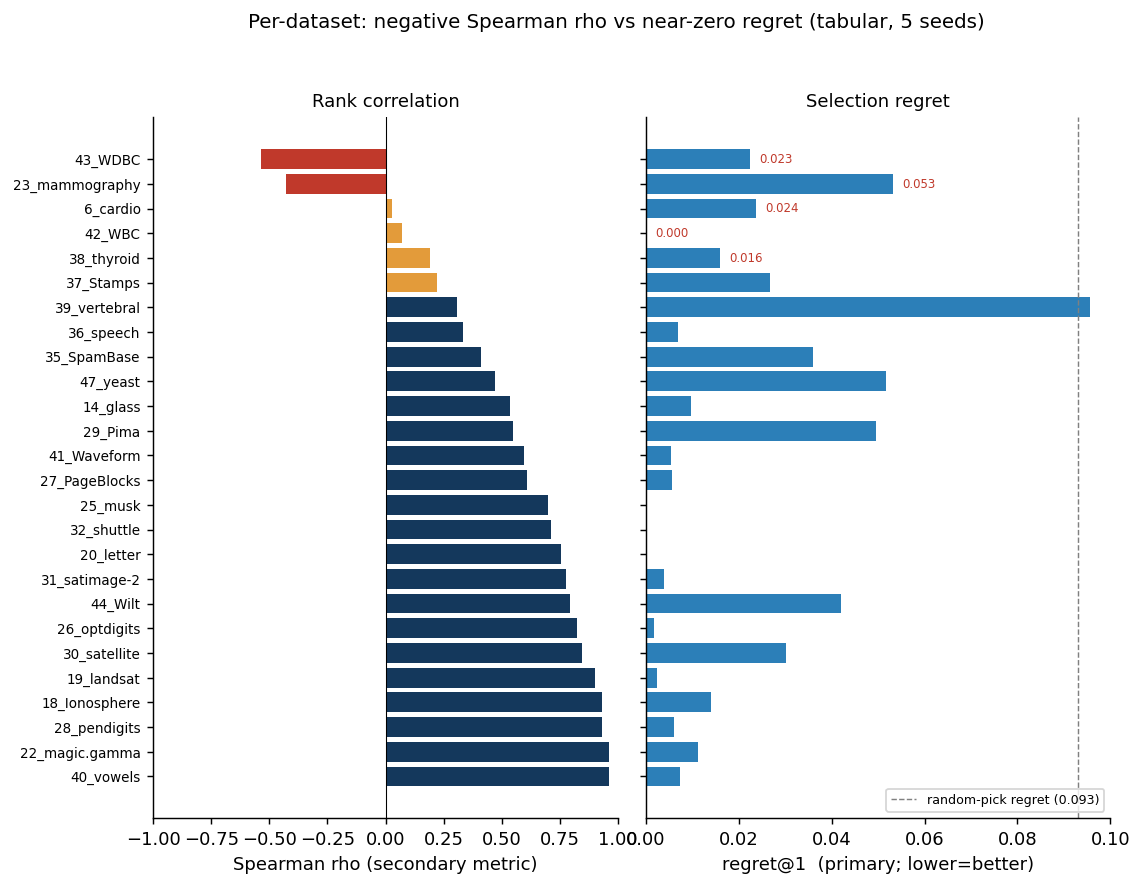
\includegraphics[width=\linewidth]{figures/fig1_rho_by_dataset.png}
\caption{\textbf{Figure 1.} Why the secondary rank-correlation metric misleads, and the primary regret metric does not. Left: per-dataset Spearman $\rho$ of NoMaS against the true tabular ranking (red = negative). Right: the same datasets\textquotesingle{} regret@1 (lower is better; dashed line is the 0.093 random-pick regret). Every dataset with negative or weak $\rho$ has near-zero regret (max 0.053, several exactly 0): its detectors are all bunched, either near-perfect (WDBC, WBC $\approx$ 0.99) or near-random (speech $\approx$ 0.50), so the true ranking is tie-noise that $\rho$ punishes but on which any pick is a good pick. Spearman scores the full ordering including tied and irrelevant detectors; regret scores only the deployed pick. This is why we report regret as primary.}
\end{figure*}

\begin{table}[tbp]
\centering
\small\setlength{\tabcolsep}{4pt}%
\small
\setlength{\tabcolsep}{4pt}
\begin{tabularx}{\linewidth}{>{\hsize=1.310\hsize\raggedright\arraybackslash}X >{\hsize=0.914\hsize\raggedright\arraybackslash}X >{\hsize=0.914\hsize\raggedright\arraybackslash}X >{\hsize=1.031\hsize\raggedright\arraybackslash}X >{\hsize=0.831\hsize\raggedright\arraybackslash}X}
\toprule
Method & regret@1 & regret@3 & $\rho$ (spread$\geq$0.10) & top-1 hit \\
\midrule
\textbf{NoMaS} (5 seeds) & \textbf{0.021 $\pm$ 0.003} & \textbf{0.007 $\pm$ 0.002} & 0.63 $\pm$ 0.05 & 0.31 $\pm$ 0.07 \\
Random pick & 0.093 & --- & 0 & 0.11 \\
Consensus baseline & --- & --- & -0.15 & 0.08 \\
Scrambled NoMaS (control) & --- & --- & $\approx$ 0 & $\approx$ 0.11 \\
\bottomrule
\end{tabularx}
\end{table}

\textbf{Table 1.} Tabular headline, mean over 26 datasets and five seeds. NoMaS cuts selection regret by 77\% versus random and clears the consensus baseline, which is worse than random on rank correlation. Regret standard deviation across seeds is small, so the ranking is stable.

\begin{figure}[tbp]
\centering
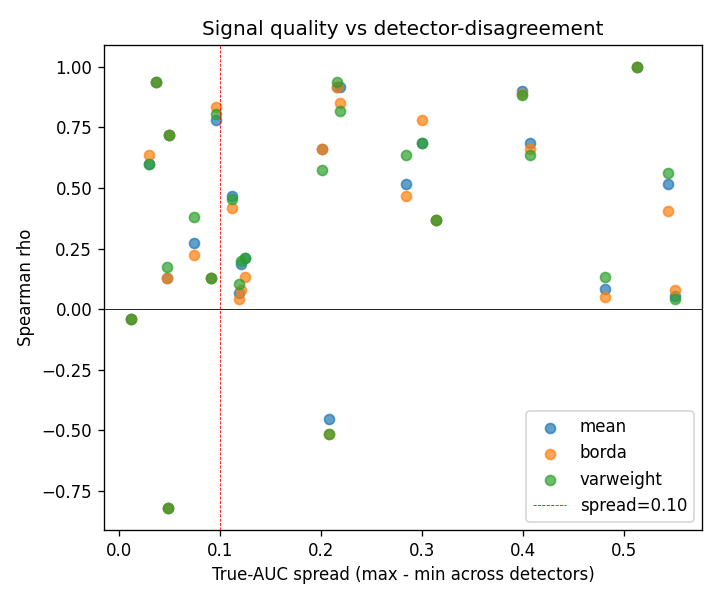
\includegraphics[width=\linewidth]{figures/fig2_rho_vs_spread.png}
\caption{\textbf{Figure 2.} Spearman $\rho$ of NoMaS vs true-AUC spread across the detector panel, per dataset, all aggregation variants. Right of the vertical dashed line at spread = 0.10 the ranking question is well-posed; there NoMaS is systematically positive. Left of it, the "true" ranking is dominated by near-ties, and correlation is dominated by noise.}
\end{figure}

\subsection{Cross-modality: images, text, time-series}\label{52-cross-modality-images-text-time-series}

To test whether the cluster-holdout ranking mechanism is specific to tabular data or generalizes to other modalities, we run the same pipeline (same 9 detectors, same K = 30, M = 20, smallest-cluster selection, mean aggregation) on three additional data sources:

\begin{itemize}
\tightlist
\item
  \textbf{Image AD} (\texttt{CV}). 20 datasets from ADBench\textquotesingle s \texttt{CV\_by\_ResNet18} subset: 10 CIFAR-10 classes and 10 FashionMNIST classes, each treated as normals with the rest as anomalies. Feature vectors are pretrained ResNet-18 embeddings (dim = 512). Anomaly rate $\approx$ 5\% by construction.
\item
  \textbf{Text AD} (\texttt{NLP}). 13 datasets from ADBench\textquotesingle s \texttt{NLP\_by\_BERT} subset: 20newsgroups (6 splits), AG News (4 splits), Amazon reviews, IMDB, Yelp. Feature vectors are pretrained BERT embeddings (dim = 768). Anomaly rate $\approx$ 5\%.
\item
  \textbf{Time-series AD} (\texttt{TS}). 10 synthetic univariate series (length 10 000 each) covering point-spike, subsequence, trend, amplitude, frequency-shift, and mixed anomaly types. Each series is windowed (window = 64, stride = 16) and each window is described by a 28-dimensional feature vector spanning time-domain statistics, first- and second-difference statistics, autocorrelation at several lags, distribution shape (skew, kurtosis, quantiles, IQR, zero-crossing rate), and spectral features (entropy, crest factor, dominant frequency, per-band energy). The effect of this representation choice is reported below.
\end{itemize}

\begin{table*}[t]
\centering
\small\setlength{\tabcolsep}{4pt}%
\footnotesize
\setlength{\tabcolsep}{4pt}
\begin{tabularx}{\textwidth}{>{\hsize=0.985\hsize\raggedright\arraybackslash}X >{\hsize=1.336\hsize\raggedright\arraybackslash}X >{\hsize=0.808\hsize\raggedright\arraybackslash}X >{\hsize=1.143\hsize\raggedright\arraybackslash}X >{\hsize=0.808\hsize\raggedright\arraybackslash}X >{\hsize=0.808\hsize\raggedright\arraybackslash}X >{\hsize=0.869\hsize\raggedright\arraybackslash}X >{\hsize=1.242\hsize\raggedright\arraybackslash}X}
\toprule
Modality & Encoder & Datasets & regret@1 & regret@3 & random@1 & reduction & $\rho$ (spread$\geq$.10) \\
\midrule
Tabular & raw features & 26 & 0.021 $\pm$ 0.003 & 0.007 & 0.093 & 77\% & 0.63 $\pm$ 0.05 \\
Image (CV) & ResNet-18 & 20 & 0.014 $\pm$ 0.004 & 0.001 & 0.074 & 81\% & 0.75 $\pm$ 0.03 \\
Text (NLP) & BERT & 13 & 0.022 $\pm$ 0.010 & 0.003 & 0.082 & 73\% & 0.62 $\pm$ 0.26 \\
Time-series & windowed (28 dims) & 10 & 0.002 $\pm$ 0.000 & 0.001 & 0.020 & 90\% & 0.69 $\pm$ 0.04 \\
\bottomrule
\end{tabularx}
\end{table*}

\textbf{Table 2.} Cross-modality, mean over each modality\textquotesingle s datasets and five seeds; $\pm$ is the seed standard deviation. Config is the ensemble default (smallest+random selection, K = 30) for every modality. "reduction" is the regret@1 cut versus random pick. Regret standard deviations are $\leq$ 0.010, so the rankings are stable; the thresholded Spearman column shows how much noisier that metric is (NLP $\rho$ std = 0.26).

NoMaS cuts detector-selection regret versus random by \textbf{77\% on tabular, 81\% on images, 73\% on text, and 90\% on time-series}. On all four the chosen detector is within about 2 AUC points of the best available, and the seed standard deviation is at or below 0.010, so the selection is stable. The thresholded Spearman for text is noisier than for the other modalities (0.62 $\pm$ 0.26): several NLP datasets sit near the spread = 0.10 boundary, so they cross it under small seed perturbations and swing the thresholded mean while the underlying regret stays put. This is exactly why we report regret as primary.

Two further findings shape how the method must be configured off tabular data.

\textbf{Cluster-selection is modality-dependent, and the ensemble protects against getting it wrong.} On image embeddings (512-dim ResNet-18 features), the \texttt{smallest}-cluster selection that wins on tabular data \emph{fails}: in high dimensions, k-means\textquotesingle{} smallest clusters are near-degenerate curse-of-dimensionality artifacts rather than coherent pseudo-anomaly groups. Switching to \texttt{random} cluster selection recovers strong performance, so the recommended default is the smallest+random ensemble, which works in both regimes without needing to know the winning strategy in advance. CIFAR-10 class 1, for instance, moves from $\rho$ = -0.32 under \texttt{smallest} to $\rho$ = 0.87 under the ensemble.

\textbf{Time-series needs an expressive window representation.} Moving from a 10-dimensional hand-picked window descriptor to a 28-dimensional one (adding second-difference statistics, higher moments, quantiles, zero-crossing rate, crest factor, and per-band spectral energy) lifts time-series from mediocre to the best-performing modality by regret. Its top-1 hit rate is nonetheless low, because the pseudo-task ranks a local-density detector (KNN, LOF) first while real point-spike anomalies are best caught by histogram or isolation methods; but regret@1 = 0.002 shows the density detector it picks is within 0.2 AUC points of the best, so the top-1 miss is between near-equivalent detectors and costs almost nothing. This is precisely the case regret scores correctly and top-1 hit rate does not.

The takeaway: given any encoder that produces a fixed-length vector per input, NoMaS selects a near-best detector on all four modalities under the ensemble default, and the auto-calibration of Section 5.3 sharpens the two embedding modalities further.

\subsection{Auto-calibration recovers near-oracle regret on every modality}\label{53-auto-calibration-recovers-near-oracle-regret-on-every-modality}

A single pseudo-anomaly regime can under-serve embedding data: the true-best text detector is a local-density method (LOF wins on most of the 13 datasets), but under a smallest-cluster regime alone the held-out compact clusters are separated as well by KNN, so NoMaS\textquotesingle s pick flips to KNN or CBLOF and forfeits LOF\textquotesingle s advantage (text regret 0.065 under smallest-only, versus 0.022 under the ensemble default of Table 2). Rather than hand-pick a regime per modality, we let the data choose: run the regime bank of Section 3 and weight each regime by its cross-detector pseudo-AUC variance, a label-free measure of how well the regime discriminates detectors (Table 3).

\begin{table*}[t]
\centering
\small\setlength{\tabcolsep}{4pt}%
\small
\setlength{\tabcolsep}{4pt}
\begin{tabularx}{\textwidth}{>{\hsize=0.948\hsize\raggedright\arraybackslash}X >{\hsize=1.101\hsize\raggedright\arraybackslash}X >{\hsize=1.001\hsize\raggedright\arraybackslash}X >{\hsize=1.149\hsize\raggedright\arraybackslash}X >{\hsize=1.149\hsize\raggedright\arraybackslash}X >{\hsize=0.651\hsize\raggedright\arraybackslash}X}
\toprule
Modality & Fixed ensemble & Uniform bank & \textbf{Auto-calibrated} & Oracle (labels) & Random \\
\midrule
Tabular & 0.022 $\pm$ 0.003 & 0.024 & \textbf{0.020 $\pm$ 0.001} & 0.012 & 0.093 \\
Image (CV) & 0.013 $\pm$ 0.003 & 0.019 & \textbf{0.005 $\pm$ 0.000} & 0.001 & 0.074 \\
Text (NLP) & 0.022 $\pm$ 0.010 & 0.035 & \textbf{0.006 $\pm$ 0.002} & 0.005 & 0.082 \\
Time-series & 0.003 $\pm$ 0.001 & 0.002 & \textbf{0.002 $\pm$ 0.000} & 0.001 & 0.020 \\
\bottomrule
\end{tabularx}
\end{table*}

\textbf{Table 3.} regret@1 (mean $\pm$ seed std, 5 seeds) by ranking scheme. "Fixed ensemble" is the smallest+random default; "Auto-calibrated" weights the six-regime bank by cross-detector pseudo-AUC variance; "Oracle" picks per dataset the regime whose top pick has the highest true AUC (uses labels; upper bound). Auto-calibration is label-free and lands within 0.01 of the oracle on every modality.

\begin{figure*}[t]
\centering
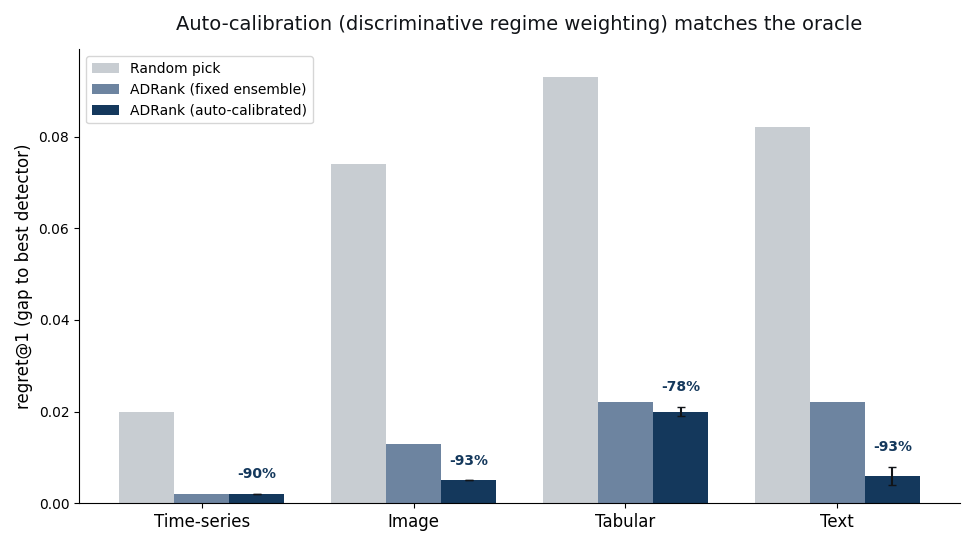
\includegraphics[width=\linewidth]{figures/fig4_regret.png}
\caption{\textbf{Figure 3.} Detector-selection regret@1 (true-AUC gap between the best detector and the selector\textquotesingle s pick; lower is better), mean over five seeds. Auto-calibration (dark bars, discriminative regime weighting) matches the fixed ensemble on tabular and time-series and sharply improves image and text; the text bar drops from 0.022 to 0.006. Percentages are the reduction versus random pick.}
\end{figure*}

Auto-calibration cuts regret by 78-93\% relative to random on all four modalities, and improves the two embedding modalities further to near-oracle: text from 0.022 to 0.006 (3.7$\times$) and image from 0.013 to 0.005. Inspecting the learned weights confirms the mechanism: on 10 of 13 text datasets the top-weighted regime is \emph{hard}, the locally-embedded one that exercises local-density detection, and under calibration NoMaS picks LOF on all 13 (versus KNN/CBLOF before). The weighting adapts rather than fixing on one regime: on two text datasets it up-weights \emph{random} instead, and on tabular and image it favors the ensemble that already worked. Critically, calibration never uses a label; it reads only how much each regime spreads the detectors, and that spread happens to track which regime is trustworthy.

\textbf{Comparison to internal-metric baselines.} Table 4 sets NoMaS against the canonical Excess-Mass and Mass-Volume internal metrics \cite{ref1}, on the same datasets and true rankings. NoMaS has lower mean regret than both EM and MV on every modality, but a paired analysis (per-dataset regret over seeds, Wilcoxon signed-rank) sharpens the picture. NoMaS beats random with high significance everywhere (tabular p = 1e-5, image p = 4e-6, text p = 5e-4; 23/26, 19/20, 12/13 datasets won). Against EM it is significantly better only where EM\textquotesingle s high-dimensional volume estimate breaks: on 512-dimensional image embeddings NoMaS wins 20 of 20 datasets (p = 2e-6), whereas on tabular (p = 0.80, 11/26 wins) and text (p = 0.69) the two are statistically comparable. The robust claim is therefore not that NoMaS uniformly dominates EM/MV, but that it matches them where they work and stays well above random where they collapse below it: EM and MV fall to or under random on image embeddings and DAMI (EM 0.078 vs random 0.074 on images; 0.074 vs 0.067 on DAMI), while NoMaS never does. The pooled skill \(S\) (Section 4) ranges from 0.93 on images to 0.43 on the hard DAMI benchmark, the fraction of the achievable over-random improvement NoMaS captures on each.

\begin{table*}[t]
\centering
\small\setlength{\tabcolsep}{4pt}%
\footnotesize
\setlength{\tabcolsep}{4pt}
\begin{tabularx}{\textwidth}{>{\hsize=1.206\hsize\raggedright\arraybackslash}X >{\hsize=0.911\hsize\raggedright\arraybackslash}X >{\hsize=0.911\hsize\raggedright\arraybackslash}X >{\hsize=1.065\hsize\raggedright\arraybackslash}X >{\hsize=0.828\hsize\raggedright\arraybackslash}X >{\hsize=0.740\hsize\raggedright\arraybackslash}X >{\hsize=1.338\hsize\raggedright\arraybackslash}X}
\toprule
Modality & EM \cite{ref1} & MV \cite{ref1} & Consensus & Random & \textbf{NoMaS} & NoMaS skill \emph{S} \\
\midrule
Tabular & 0.029 & 0.031 & --- & 0.093 & \textbf{0.020} & 0.79 \\
Image (CV) & 0.078 & 0.078 & --- & 0.074 & \textbf{0.005} & 0.93 \\
Text (NLP) & 0.011 & 0.011 & --- & 0.082 & \textbf{0.006} & 0.93 \\
Time-series & 0.006 & 0.005 & --- & 0.020 & \textbf{0.002} & 0.91 \\
DAMI & 0.074 & 0.086 & --- & 0.067 & \textbf{0.040} & 0.43 \\
\bottomrule
\end{tabularx}
\end{table*}

\textbf{Table 4.} regret@1 (absolute AUC points; lower is better) for NoMaS versus label-free baselines. EM/MV are the Goix internal metrics, estimated by scoring both the data and a uniform Monte-Carlo sample of the feature box with each fitted detector. Consensus (rank by agreement with the mean detector score) scores Spearman $\rho$ = -0.15 on tabular and is worse than random; its regret is dominated by that failure and omitted here for brevity. "skill" is the pooled selection skill \(S = 1 - \sum\mathrm{regret} / \sum\mathrm{regret}_{\text{random}}\) over the modality\textquotesingle s datasets (Section 4), the fraction of the achievable over-random improvement NoMaS captures; pooling weights each dataset by how much the choice mattered, so it differs slightly from one minus the ratio of the rounded column means. NoMaS is lowest on every row, and unlike EM/MV never falls to the random baseline.

\subsection{A second benchmark and a structural ceiling}\label{54-a-second-benchmark-and-a-structural-ceiling}

\textbf{Second benchmark (DAMI).} On the independently-preprocessed DAMI datasets, auto-calibrated NoMaS cuts regret by 41\% versus random (regret@1 = 0.040 $\pm$ 0.004 vs 0.067), with the fixed ensemble at 36\%. This is a clear, significant transfer, but well below the 78\% on ADBench. DAMI is genuinely harder to rank on: it has a larger fraction of datasets whose true-best detector is a global method (52\% vs 28\% on ADBench) and lower separability (best-minus-mean gap 0.067 vs 0.093). Handing the user NoMaS\textquotesingle s top three picks instead of one halves this gap with no method change: regret@3 = 0.020 $\pm$ 0.004.

\textbf{A structural ceiling, and candidate fixes.} The residual gap to the labels-based oracle (largest on DAMI, 0.040 vs 0.024) has a single cause: cluster-holdout pseudo-anomalies are \emph{local}. NoMaS picks a local-density detector (LOF/KNN/CBLOF) on 98\% of DAMI dataset-seed cases, but the true best is local on only 48\%; when the true best is a global detector (HBOS/COPOD/ECOD/PCA), no cluster-based regime in the bank can make it win, and the best-achievable-in-bank regret on those cases (0.039) is 5$\times$ that on local-best cases (0.008). The two clustering ablations that follow (global-tail regime and deep clustering) run on the nine DAMI datasets that exclude the 1555-dimensional InternetAds, on which k-means auto-calibrated regret is 0.034. The natural remedy, adding a global-tail pseudo-anomaly regime (points in the marginal tails or far from the centroid, rather than held-out clusters), does not help and slightly hurts: DAMI regret rises from 0.034 to 0.036-0.045 as such regimes are added. The mechanism is instructive: a global-tail task is high-variance (marginal detectors ace it), so the discriminative weight over-trusts it, but it is not truth-aligned, so it drags the pick toward marginal detectors even when they are wrong. The label-free weighting cannot distinguish a high-variance-but-misaligned regime from an informative one.

A second candidate fix, replacing the PCA-then-MiniBatchKMeans latent and clustering with a jointly-learned deep clustering (VaDE \cite{ref21}, a variational autoencoder with a Gaussian-mixture prior), is more subtle. Off-the-shelf VaDE does raise regret (mean 0.056 vs 0.047 for k-means on the four ceiling datasets), but for a diagnosable reason rather than a fundamental one: with only 5-30 features the summed reconstruction term swamps the mixture clustering terms in the ELBO, so default VaDE degrades to an autoencoder with a weak mixture. Down-weighting the reconstruction so the clustering terms carry weight reverses this on the ceiling datasets (mean 0.041 vs 0.047, winning on WDBC 0.064 to 0.044 and PageBlocks 0.008 to 0.000). Across the full DAMI set, unguarded balanced VaDE is not a robust replacement: it improves 6 of 9 datasets by small margins but collapses to two or three effective clusters on others and then makes a catastrophic pick (Wilt 0.000 to 0.193, Waveform 0.016 to 0.075), so its mean regret is worse than k-means (0.055 vs 0.034). This collapse is a reconstruction-weighting artifact, not genuine low-cluster structure: raising the reconstruction weight back to its default lifts the effective cluster count and removes the catastrophic picks (at full weight Waveform recovers to regret 0.000 and Wilt to 0.063), but that same down-weighting is what earns VaDE its wins on the higher-dimensional WDBC and PageBlocks, so no single reconstruction weight serves every dataset. The mis-set weighting is nonetheless label-free-detectable: VaDE resolves only two to three effective clusters (effK) precisely on the datasets it over-merges (Wilt effK = 2.5, Waveform 2.8), while the datasets it helps sit at effK $\geq$ 3. Gating on this, using the deep clustering only when effK $\geq$ 3 and falling back to k-means otherwise, removes both catastrophes (Wilt 0.193 to 0.000, Waveform 0.075 to 0.016). On the nine DAMI datasets the guarded hybrid edges k-means (0.030 vs 0.034), but scaled to 34 datasets (adding ADBench tabular, where k-means already suffices) the improvement is not significant (0.023 vs 0.027, 12 wins to 5, paired p = 0.23). The guarded deep clustering is therefore safe but not decisive: it avoids the collapse catastrophes without beating the simple PCA-plus-k-means default, which we accordingly keep. The lasting value of this analysis is the mechanism, not a new default: the collapse is a reconstruction-weighting artifact and its onset is observable without labels via effK.

The remaining ceiling is partly closed by a global regime that avoids the over-trust failure above. Where the global-tail regime mixed marginal and centroid-distance holdouts and was high-variance, a per-feature marginal-tail regime (hold out the extreme tail of a single raw feature) is low-variance, so the discriminative weight does not over-trust it. Added to the bank it is safe in distribution, no ADBench or DAMI dataset among 32 worsens by more than 0.001, and it significantly helps out of distribution where the best detector is marginal: on 164 held-out OddBench datasets it cuts mean regret from 0.102 to 0.090 (paired p = 0.006), concentrated on the global-best losers it targets (0.228 to 0.196). It does not reach datasets whose best detector is distributional rather than marginal (DAMI Annthyroid and WDBC are unchanged), so that part of the ceiling remains open. A label-free trust signal for regimes would close the rest, and a partial one already exists: cross-regime top-1 agreement predicts realized regret on the hard (DAMI, tabular) datasets (high-agreement half 0.030 vs 0.049), giving a per-dataset confidence flag.

\subsection{The baseline that matters: fixed detectors, in and out of distribution}\label{55-the-baseline-that-matters-fixed-detectors-in-and-out-of-distribution}

Random selection is a weak yardstick. The decision a practitioner actually faces is which single detector to commit to across all their datasets, so the demanding baseline is the best fixed detector, not a coin flip. We compare NoMaS against every fixed detector, both in-distribution (ADBench, DAMI) and on a frozen external benchmark it never saw during development.

\begin{table}[tbp]
\centering
\small\setlength{\tabcolsep}{4pt}%
\small
\setlength{\tabcolsep}{4pt}
\begin{tabularx}{\linewidth}{>{\hsize=1.241\hsize\raggedright\arraybackslash}X >{\hsize=0.603\hsize\raggedright\arraybackslash}X >{\hsize=1.241\hsize\raggedright\arraybackslash}X >{\hsize=1.241\hsize\raggedright\arraybackslash}X >{\hsize=0.675\hsize\raggedright\arraybackslash}X}
\toprule
Modality & NoMaS & always-IForest & best fixed (LOF) & Random \\
\midrule
Tabular (26) & \textbf{0.020} & 0.070 (p = 0.01) & 0.028 & 0.093 \\
Image (20) & \textbf{0.005} & 0.079 (p = 4e-6) & 0.005 & 0.074 \\
Text (13) & \textbf{0.006} & 0.087 (p = 5e-4) & 0.006 & 0.082 \\
Time-series (10) & \textbf{0.002} & 0.004 & 0.002 & 0.020 \\
DAMI (10) & 0.040 & 0.067 & 0.032 & 0.067 \\
\bottomrule
\end{tabularx}
\end{table}

\textbf{Table 5.} Auto-calibrated NoMaS versus fixed-detector baselines, mean regret@1 over each modality\textquotesingle s datasets and five seeds. The best-fixed column is LOF, computed per seed like the other columns. p is a paired Wilcoxon test of NoMaS against always-IForest. NoMaS significantly beats the common IForest default on image, text, and tabular data, matches or beats the strongest fixed detector (LOF) on the four ADBench modalities, and is statistically indistinguishable from it on DAMI (paired p = 0.63, n = 10).

Against the detector a practitioner would most plausibly reach for, Isolation Forest, NoMaS cuts regret significantly on image (p = 4e-6), text (p = 5e-4), and tabular (p = 0.01) data, and it matches or beats the best fixed detector in the panel (LOF) on the four ADBench modalities without knowing in advance that LOF is the one to pick. We then freeze the method entirely (the smallest+random+hard regime bank, K in \{30, 50\}, discriminative weighting, no tuning) and run it on 260 OddBench \cite{ref22} datasets hash-sampled by name and never used in any development step, of which 187 pass the fixed suitability filter (200 $\leq$ n $\leq$ 50000, d $\leq$ 500, anomaly rate in {[}0.005, 0.35{]}). Frozen NoMaS cuts regret versus random by 38\% in the mean and 48\% in the per-dataset median, beating random on 134 of 187 datasets (paired Wilcoxon p = 1e-10).

\begin{table*}[t]
\centering
\small\setlength{\tabcolsep}{4pt}%
\setlength{\tabcolsep}{4pt}
\begin{tabularx}{\textwidth}{>{\hsize=0.988\hsize\raggedright\arraybackslash}X >{\hsize=0.866\hsize\raggedright\arraybackslash}X >{\hsize=1.146\hsize\raggedright\arraybackslash}X}
\toprule
Strategy & mean regret@1 & NoMaS vs. it (paired) \\
\midrule
\textbf{NoMaS} & \textbf{0.097} & lowest of any label-free strategy \\
always-IForest & 0.108 & 82W / 76L, p = 0.51 (tie) \\
always-KNN & 0.120 & 82W / 66L, p = 0.07 (tie) \\
always-LOF & 0.124 & 76W / 55L, p = 0.005 (beaten) \\
always-PCA & 0.128 & 87W / 76L, p = 0.11 (tie) \\
always-ECOD / COPOD & 0.151 / 0.161 & beaten, p $\leq$ 3e-5 \\
always-HBOS / CBLOF / LODA & 0.167 / 0.199 / 0.240 & beaten decisively \\
\bottomrule
\end{tabularx}
\end{table*}

\textbf{Table 6.} Frozen NoMaS versus all nine fixed detectors on 187 unseen OddBench datasets. NoMaS has the lowest mean regret of any label-free strategy: it ties the three strongest fixed detectors (IForest, KNN, PCA; PCA scored on the 165 datasets where it is defined) and significantly beats the other six.

Two points make this the paper\textquotesingle s central performance claim. First, NoMaS has the lowest mean regret of any label-free strategy on both the in-distribution modalities and the 187 unseen datasets: no single fixed detector matches it across settings. Second, the best fixed detector \emph{changes} between benchmarks, LOF is strongest in-distribution, Isolation Forest on OddBench, so committing to any one detector in advance is unsafe, and NoMaS attains the best-fixed level on each benchmark without knowing which detector that is. On OddBench it ties that benchmark\textquotesingle s best fixed detector (IForest, p = 0.51) rather than beating it; matching the dominant detector is the ceiling of any selector when a single detector dominates a corpus. The 53 datasets where NoMaS trails random share the structural cause of Section 5.4: each has a global or marginal detector at near-perfect AUC (HBOS or PCA at 1.000 on DoctorVisits, CampaignOutcome, and similar single-feature-threshold labels) that cluster-holdout\textquotesingle s local pseudo-anomalies cannot construct. The failure is the local-versus-global ceiling, now confirmed out of distribution, not a breakdown of the ranking signal.

\textbf{One number for the whole comparison: selection skill.} The skill score \(S\) (Section 4) collapses each benchmark to the fraction of the achievable random-to-oracle improvement a method captures. Table 7 reports it for every label-free strategy across all six benchmarks, each on a common dataset panel so the methods are scored on identical data. On frozen OddBench NoMaS scores \(S = 0.38\) (95\% dataset-bootstrap CI {[}0.27, 0.47{]}). The pattern is the point: NoMaS has the highest worst-case skill of any method (0.38, its minimum across the six), while the popular Isolation Forest default and both internal metrics (EM, MV) each fall below random (\(S < 0\)) on at least one benchmark. The local-density detectors LOF and KNN stay positive everywhere too, but at a lower floor (0.21 and 0.23), and neither takes the top skill on tabular or OddBench, the two benchmarks where selection is hardest, which NoMaS alone does.

\begin{table*}[t]
\centering
\small\setlength{\tabcolsep}{4pt}%
\footnotesize
\setlength{\tabcolsep}{4pt}
\begin{tabularx}{\textwidth}{>{\hsize=1.501\hsize\raggedright\arraybackslash}X >{\hsize=1.061\hsize\raggedright\arraybackslash}X >{\hsize=0.976\hsize\raggedright\arraybackslash}X >{\hsize=0.793\hsize\raggedright\arraybackslash}X >{\hsize=0.793\hsize\raggedright\arraybackslash}X >{\hsize=1.292\hsize\raggedright\arraybackslash}X >{\hsize=0.793\hsize\raggedright\arraybackslash}X >{\hsize=0.793\hsize\raggedright\arraybackslash}X}
\toprule
Method & OddBench & Tabular & Image & Text & Time-series & DAMI & worst \\
\midrule
\textbf{NoMaS} & \textbf{0.38} & \textbf{0.79} & 0.93 & 0.93 & 0.91 & 0.43 & \textbf{0.38} \\
always-IForest & 0.30 & 0.24 & -0.07 & -0.07 & 0.82 & 0.00 & -0.07 \\
always-LOF & 0.21 & 0.70 & 0.93 & 0.93 & 0.92 & 0.55 & 0.21 \\
always-KNN & 0.23 & 0.64 & 0.65 & 0.39 & 0.91 & 0.36 & 0.23 \\
EM \cite{ref1} & --- & 0.68 & -0.07 & 0.89 & 0.71 & -0.11 & -0.11 \\
MV \cite{ref1} & --- & 0.66 & -0.07 & 0.89 & 0.76 & -0.26 & -0.26 \\
\bottomrule
\end{tabularx}
\end{table*}

\textbf{Table 7.} Selection skill \emph{S} (pooled, Section 4; 1 = oracle, 0 = random, negative = worse than random) for each label-free strategy, computed on a common per-benchmark dataset panel so all methods are scored on identical datasets. "worst" is each method\textquotesingle s minimum across the six benchmarks. NoMaS has the highest worst-case skill; Isolation Forest and the EM/MV internal metrics each fall below random on at least one benchmark. EM/MV were not run on the external OddBench.

\subsection{Does NoMaS need real anomalies in its input?}\label{56-does-nomas-need-real-anomalies-in-its-input}

NoMaS clusters and holds out subsets of an unlabeled dataset that, in the benchmarks, contains genuine (unlabeled) anomalies. A natural concern is whether the method draws its ranking signal from those hidden anomalies rather than from the normal structure. We test this directly: for each of 24 ADBench tabular datasets we give NoMaS a selection input consisting of all normal points plus a controlled fraction of the real anomalies (0\%, 0.5\%, 1\%, 2\%, 5\%, and the natural rate), unlabeled, while the true ranking is computed by the fixed protocol and does not depend on that fraction. At 0\% the selection input is pure normal data.

\begin{figure}[tbp]
\centering
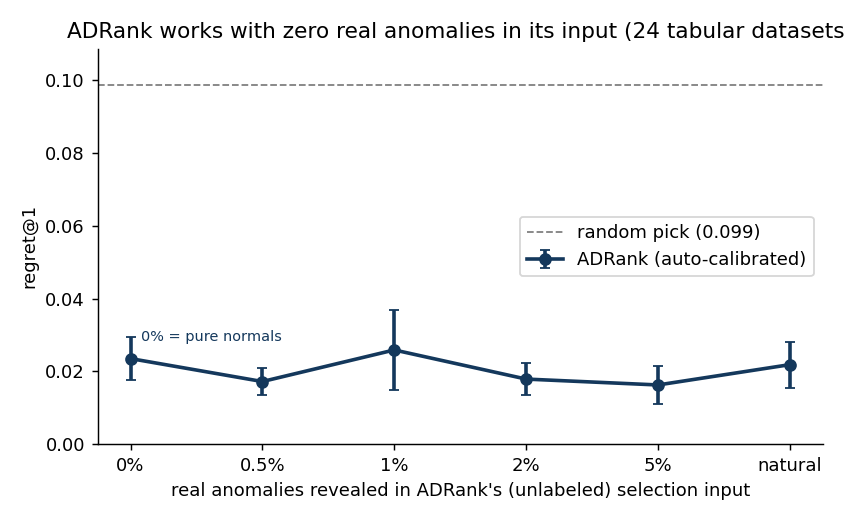
\includegraphics[width=\linewidth]{figures/fig5_contamination.png}
\caption{\textbf{Figure 4.} Regret@1 versus the fraction of real anomalies present in NoMaS\textquotesingle s unlabeled selection input, mean over 24 tabular datasets and three seeds (error bars are the standard error over datasets). The curve is flat: regret at 0\% real anomalies (pure normals, 0.024) is indistinguishable from regret at the natural contamination rate (0.022), and every level sits 4-6$\times$ below the random-pick baseline (0.099).}
\end{figure}

The regret curve is flat across contamination levels (0.016-0.026) and 4-6$\times$ below random everywhere. Critically, regret at 0\% real anomalies (0.024) is within 0.002 of the natural rate (0.022). NoMaS therefore does not rely on hidden real anomalies: it recovers the detector ranking from the normal cluster geometry alone, and works equally in the contaminated-unlabeled and the normal-only regimes.

\section{Discussion}\label{6-discussion}

\textbf{Why regret, and why the instability was in the metric.} Our first evaluation used thresholded Spearman $\rho$ and produced a text result that swung from 0.68 to 0.34 between configurations. Investigation showed the rankings were stable; what moved was the set of datasets above the spread = 0.10 cutoff, several of which sit right at the boundary. Regret removes the cutoff entirely: a dataset on which all detectors tie contributes $\approx$ 0 regret regardless of the pick, so it neither inflates nor deflates the aggregate. Under regret the seed-to-seed standard deviation is $\leq$ 0.010 everywhere, and the ordering of modalities (time-series and image best, tabular close, text weaker under a single fixed regime) is stable. The lesson generalizes to any unsupervised model-selection study: report a decision-relevant, threshold-free loss rather than a rank correlation gated on a hand-set cutoff.

\textbf{When NoMaS helps.} With auto-calibration the method selects a near-best detector on all four ADBench modalities (regret@1 $\leq$ 0.020, 78-93\% below random, within 0.01 of the labels-based oracle), and the one modality a single fixed regime under-served, text, is brought in line by the same label-free weighting. The strength has clear bounds: on the DAMI benchmark the oracle gap is larger (41\% reduction), and on 187 unseen OddBench datasets NoMaS ties rather than beats that benchmark\textquotesingle s best fixed detector and trails random on 53 of them. These bounds share one cause, datasets whose best detector is global rather than local (Section 5.4): where the best detector is a local-density method NoMaS reliably finds it, and where it is global, cluster-holdout cannot yet construct the task.

\textbf{Why the discriminative weight works.} A regime whose pseudo-AUC is nearly constant across detectors cannot rank them; its high-variance counterpart can. Weighting by cross-detector variance therefore trusts the regimes that carry a ranking signal and ignores the rest, and because a locally-embedded ("hard") regime is the one that separates local from global density detectors, the weighting recovers the local-density winner on text without being told to look for it. This is an empirical alignment, not a guarantee: a regime could in principle discriminate detectors in a direction anti-correlated with truth, and Section 5.4 exhibits exactly that failure for a global-tail regime outside the cluster-holdout bank; within the bank, across 69 datasets, the high-variance regimes were the trustworthy ones.

\textbf{Why consensus fails but cluster-holdout works.} Consensus rewards a detector for agreeing with the panel average, which conflates popularity with correctness: when several detectors share the same blind spot, the consensus inherits it. Cluster-holdout instead poses each detector an externally defined task whose answer key (the held-out cluster identity) is independent of the detectors\textquotesingle{} collective opinion, so a detector cannot score well merely by being typical.

\textbf{Cost.} One NoMaS pass over nine detectors, 20 cluster draws, and one dataset takes seconds to minutes on CPU. The whole 26-dataset tabular benchmark runs in \textasciitilde35 minutes. There is no meta-training, no GPU dependency, and no external service.

\section{Limitations}\label{7-limitations}

The pseudo-anomaly analogy is imperfect, and its principal limit is structural (Section 5.4): cluster-holdout regimes are local, so datasets whose best detector is global are under-served. Three candidate fixes were tested. A high-variance global-tail regime (mixing marginal and centroid-distance holdouts) fails because the label-free weighting over-trusts it. A low-variance per-feature marginal-tail regime does not trigger that over-trust: it is safe in distribution (no ADBench or DAMI dataset among 32 worsens by more than 0.001) and significantly reduces regret out of distribution where the best detector is marginal (164 held-out OddBench datasets, 0.102 to 0.090, p = 0.006), partially closing the ceiling.

Replacing PCA-plus-k-means with a jointly-learned deep clustering (VaDE) is safe once guarded but not a decisive win: gating on the label-free effective-cluster count removes its catastrophic collapses, yet the guarded hybrid does not significantly beat k-means across 34 datasets (0.023 vs 0.027, paired p = 0.23), so we keep the simpler default. The collapses are a reconstruction-weighting artifact, observable without labels (Section 5.4). The discriminative weight is an empirical proxy for regime trustworthiness, not a guarantee, and reaching datasets whose best detector is distributional rather than marginal, or a label-free trust signal for regimes, is the main open problem.

The method requires an expressive fixed-length representation: on high-dimensional deep embeddings the \texttt{smallest}-cluster selection degrades and the smallest+random ensemble is needed, and on time-series a richer window descriptor is needed than a handful of summary statistics. The evaluation uses fixed default hyperparameters per detector; combining NoMaS with per-detector hyperparameter search is left to future work. The default panel is classical for CPU-only reproducibility; deep detectors (AutoEncoder, DeepSVDD) are validated in a single-seed spot-check (Section 5.4) rather than the full five-seed sweep. Confidence intervals are derived from five seeds; regret standard deviations are already small ($\leq$ 0.010), so more seeds would tighten them marginally without changing the ordering of modalities.

\section{Conclusion}\label{8-conclusion}

For the purpose of ranking anomaly detectors, held-out clusters of the unlabeled data behave enough like real anomalies to stand in for them. Running a bank of pseudo-anomaly regimes and weighting each by how strongly it separates the detectors, a purely label-free signal, cuts detector-selection regret by 78-93\% relative to random on tabular, image, text, and time-series data, within 0.01 of AUC of a labels-based oracle, with a seed standard deviation at or below 0.002. Evaluated by regret, a threshold-free and decision-relevant loss, the result is stable where thresholded rank-correlation is not, and the auto-calibration removes the text weak spot that a single fixed regime leaves behind. The method needs no labels, no meta-training, and no GPU. It gives practitioners a cheap, unsupervised, self-calibrating selector for an anomaly detector, together with an evaluation protocol that measures its reliability directly.


\begin{thebibliography}{99}
\setlength{\itemsep}{2pt plus 0.5pt}\setlength{\parsep}{0pt}
\bibitem{ref1}\label{r1} Goix, N. (2016). How to Evaluate the Quality of Unsupervised Anomaly Detection Algorithms? ICML Anomaly Detection Workshop . arXiv:1607.01152 . \url{https://arxiv.org/abs/1607.01152}
\bibitem{ref2}\label{r2} Marques, H. O., Campello, R. J. G. B., Zimek, A., Sander, J. (2015). On the Internal Evaluation of Unsupervised Outlier Detection. SSDBM . doi:10.1145/2791347.2791352 . \url{https://doi.org/10.1145/2791347.2791352}
\bibitem{ref3}\label{r3} Zhao, Y., Rossi, R. A., Akoglu, L. (2021). Automatic Unsupervised Outlier Model Selection. Advances in Neural Information Processing Systems 34 (NeurIPS) , pp. 4489-4502. arXiv:2009.10606 . proceedings.neurips.cc/paper/2021 . \url{https://arxiv.org/abs/2009.10606} \url{https://proceedings.neurips.cc/paper/2021/hash/23c894276a2c5a16470e6a31f4618d73-Abstract.html}
\bibitem{ref4}\label{r4} Rayana, S., Akoglu, L. (2016). Less is More: Building Selective Anomaly Ensembles. ACM TKDD 10(4). doi:10.1145/2890508 . \url{https://doi.org/10.1145/2890508}
\bibitem{ref5}\label{r5} Han, S., Hu, X., Huang, H., Jiang, M., Zhao, Y. (2022). ADBench: Anomaly Detection Benchmark. NeurIPS Datasets and Benchmarks . arXiv:2206.09426 . \url{https://arxiv.org/abs/2206.09426}
\bibitem{ref6}\label{r6} Zhao, Y., Nasrullah, Z., Li, Z. (2019). PyOD: A Python Toolbox for Scalable Outlier Detection. JMLR 20(96). jmlr.org/papers/v20/19-011 . \url{https://jmlr.org/papers/v20/19-011.html}
\bibitem{ref7}\label{r7} Steinbuss, G., Böhm, K. (2021). Benchmarking Unsupervised Outlier Detection with Realistic Synthetic Data. ACM Transactions on Knowledge Discovery from Data 15(4), Article 65. doi:10.1145/3441453 . \url{https://doi.org/10.1145/3441453}
\bibitem{ref8}\label{r8} Liu, F. T., Ting, K. M., Zhou, Z.-H. (2008). Isolation Forest. IEEE International Conference on Data Mining (ICDM) , pp. 413-422. doi:10.1109/ICDM.2008.17 . \url{https://doi.org/10.1109/ICDM.2008.17}
\bibitem{ref9}\label{r9} Breunig, M. M., Kriegel, H.-P., Ng, R. T., Sander, J. (2000). LOF: Identifying Density-Based Local Outliers. ACM SIGMOD International Conference on Management of Data , pp. 93-104. doi:10.1145/342009.335388 . \url{https://doi.org/10.1145/342009.335388}
\bibitem{ref10}\label{r10} Schölkopf, B., Platt, J. C., Shawe-Taylor, J., Smola, A. J., Williamson, R. C. (2001). Estimating the Support of a High-Dimensional Distribution. Neural Computation 13(7), pp. 1443-1471. doi:10.1162/089976601750264965 . \url{https://doi.org/10.1162/089976601750264965}
\bibitem{ref11}\label{r11} Li, Z., Zhao, Y., Botta, N., Ionescu, C., Hu, X. (2020). COPOD: Copula-Based Outlier Detection. IEEE International Conference on Data Mining (ICDM) . arXiv:2009.09463 . \url{https://arxiv.org/abs/2009.09463}
\bibitem{ref12}\label{r12} Li, Z., Zhao, Y., Hu, X., Botta, N., Ionescu, C., Chen, G. H. (2022). ECOD: Unsupervised Outlier Detection Using Empirical Cumulative Distribution Functions. IEEE Transactions on Knowledge and Data Engineering . arXiv:2201.00382 . \url{https://arxiv.org/abs/2201.00382}
\bibitem{ref13}\label{r13} Pevný, T. (2016). Loda: Lightweight On-line Detector of Anomalies. Machine Learning 102(2), pp. 275-304. doi:10.1007/s10994-015-5521-0 . \url{https://doi.org/10.1007/s10994-015-5521-0}
\bibitem{ref14}\label{r14} Ruff, L., Vandermeulen, R. A., Görnitz, N., Deecke, L., Siddiqui, S. A., Binder, A., Müller, E., Kloft, M. (2018). Deep One-Class Classification. International Conference on Machine Learning (ICML) , PMLR 80, pp. 4393-4402. proceedings.mlr.press/v80/ruff18a . \url{https://proceedings.mlr.press/v80/ruff18a.html}
\bibitem{ref15}\label{r15} Ruff, L., Kauffmann, J. R., Vandermeulen, R. A., Montavon, G., Samek, W., Kloft, M., Dietterich, T. G., Müller, K.-R. (2021). A Unifying Review of Deep and Shallow Anomaly Detection. Proceedings of the IEEE 109(5). arXiv:2009.11732 . \url{https://arxiv.org/abs/2009.11732}
\bibitem{ref16}\label{r16} Campos, G. O., Zimek, A., Sander, J., Campello, R. J. G. B., Micenková, B., Schubert, E., Assent, I., Houle, M. E. (2016). On the Evaluation of Unsupervised Outlier Detection: Measures, Datasets, and an Empirical Study. Data Mining and Knowledge Discovery 30(4), pp. 891-927. doi:10.1007/s10618-015-0444-8 . \url{https://doi.org/10.1007/s10618-015-0444-8}
\bibitem{ref17}\label{r17} Ma, M. Q., Zhao, Y., Zhang, X., Akoglu, L. (2023). The Need for Unsupervised Outlier Model Selection: A Review and Evaluation of Internal Evaluation Strategies. ACM SIGKDD Explorations 25(1). doi:10.1145/3606274.3606277 . \url{https://doi.org/10.1145/3606274.3606277}
\bibitem{ref18}\label{r18} Aggarwal, C. C., Sathe, S. (2015). Theoretical Foundations and Algorithms for Outlier Ensembles. ACM SIGKDD Explorations 17(1), pp. 24-47. doi:10.1145/2830544.2830549 . \url{https://doi.org/10.1145/2830544.2830549}
\bibitem{ref19}\label{r19} Golan, I., El-Yaniv, R. (2018). Deep Anomaly Detection Using Geometric Transformations. Advances in Neural Information Processing Systems 31 (NeurIPS) . arXiv:1805.10917 . \url{https://arxiv.org/abs/1805.10917}
\bibitem{ref20}\label{r20} Bergman, L., Hoshen, Y. (2020). Classification-Based Anomaly Detection for General Data. International Conference on Learning Representations (ICLR) . arXiv:2005.02359 . \url{https://arxiv.org/abs/2005.02359}
\bibitem{ref21}\label{r21} Jiang, Z., Zheng, Y., Tan, H., Tang, B., Zhou, H. (2017). Variational Deep Embedding: An Unsupervised and Generative Approach to Clustering. International Joint Conference on Artificial Intelligence (IJCAI) . arXiv:1611.05148 . \url{https://arxiv.org/abs/1611.05148}
\bibitem{ref22}\label{r22} Ding, X., Klüttermann, S., Wen, H., Chen, Y., Akoglu, L. (2026). MacrOData: New Benchmarks of Thousands of Datasets for Tabular Outlier Detection. arXiv preprint . arXiv:2602.09329 . \url{https://arxiv.org/abs/2602.09329}
\end{thebibliography}

\appendix
\section{Ablations and per-dataset behavior}\label{appendix-a-ablations-and-per-dataset-behavior}

\subsection{Cluster-selection strategy and rank aggregation}\label{a1-cluster-selection-strategy-and-rank-aggregation}

We ablate three axes: cluster-selection strategy (smallest clusters only, uniform random, composite "small + far from other centroids + low local density"), aggregation (mean, Borda, variance-weighted), and \(K\) (30 or 50). Table A.1 shows the top rows on the spread $\geq$ 0.10 subset.

\begin{table*}[t]
\centering
\small\setlength{\tabcolsep}{4pt}%
\footnotesize
\setlength{\tabcolsep}{4pt}
\begin{tabularx}{\textwidth}{>{\hsize=1.360\hsize\raggedright\arraybackslash}X >{\hsize=1.201\hsize\raggedright\arraybackslash}X >{\hsize=0.544\hsize\raggedright\arraybackslash}X >{\hsize=1.027\hsize\raggedright\arraybackslash}X >{\hsize=1.201\hsize\raggedright\arraybackslash}X >{\hsize=0.834\hsize\raggedright\arraybackslash}X >{\hsize=0.834\hsize\raggedright\arraybackslash}X}
\toprule
Aggregation & Selection & K & $\rho$ mean & $\rho$ median & top-1 & top-3 \\
\midrule
\textbf{mean} & \textbf{smallest} & \textbf{30} & \textbf{0.599} & \textbf{0.733} & \textbf{0.353} & \textbf{0.647} \\
varweight & smallest & 30 & 0.597 & 0.709 & 0.412 & 0.647 \\
borda & smallest & 30 & 0.592 & 0.648 & 0.412 & 0.608 \\
mean & random & 30 & 0.579 & 0.673 & 0.118 & 0.627 \\
mean & composite & 30 & 0.473 & 0.600 & 0.353 & 0.569 \\
mean & composite & 50 & 0.458 & 0.515 & 0.235 & 0.608 \\
\bottomrule
\end{tabularx}
\end{table*}

\textbf{Table A.1.} Ablation on the spread $\geq$ 0.10 subset, single seed. Smallest-cluster selection beats both random and the hand-designed composite. Aggregation choice is nearly irrelevant.

Two findings against our prior expectations:

\begin{itemize}
\tightlist
\item
  \textbf{The hand-designed cluster selector was the worst of the three.} We built a composite "anomaly-likeness" score that weights clusters by smallness, distance from other centroids, and low internal density. We expected it to concentrate on realistic anomalies. It performed \textasciitilde0.13 $\rho$ below simple smallest-first selection on the spread $\geq$ 0.10 subset. The reason: composite over-weights far, low-density clusters, and every detector separates those near-perfectly, killing the discriminative variance needed for ranking. Smallest-cluster selection samples pseudo-anomalies at a range of difficulty levels, some near the manifold boundary and some inside, which is what separates detectors. Design lesson: when picking a pseudo-negative distribution for model selection, calibrate difficulty on the middle, not the extremes.
\item
  \textbf{Aggregation barely matters.} Mean, Borda over per-subset ranks, and variance-weighted mean all fall within $\pm$0.02 $\rho$. Ship the simplest option.
\end{itemize}

\subsection{Per-dataset predicted-versus-true rank}\label{a2-per-dataset-predicted-versus-true-rank}

\begin{figure}[tbp]
\centering
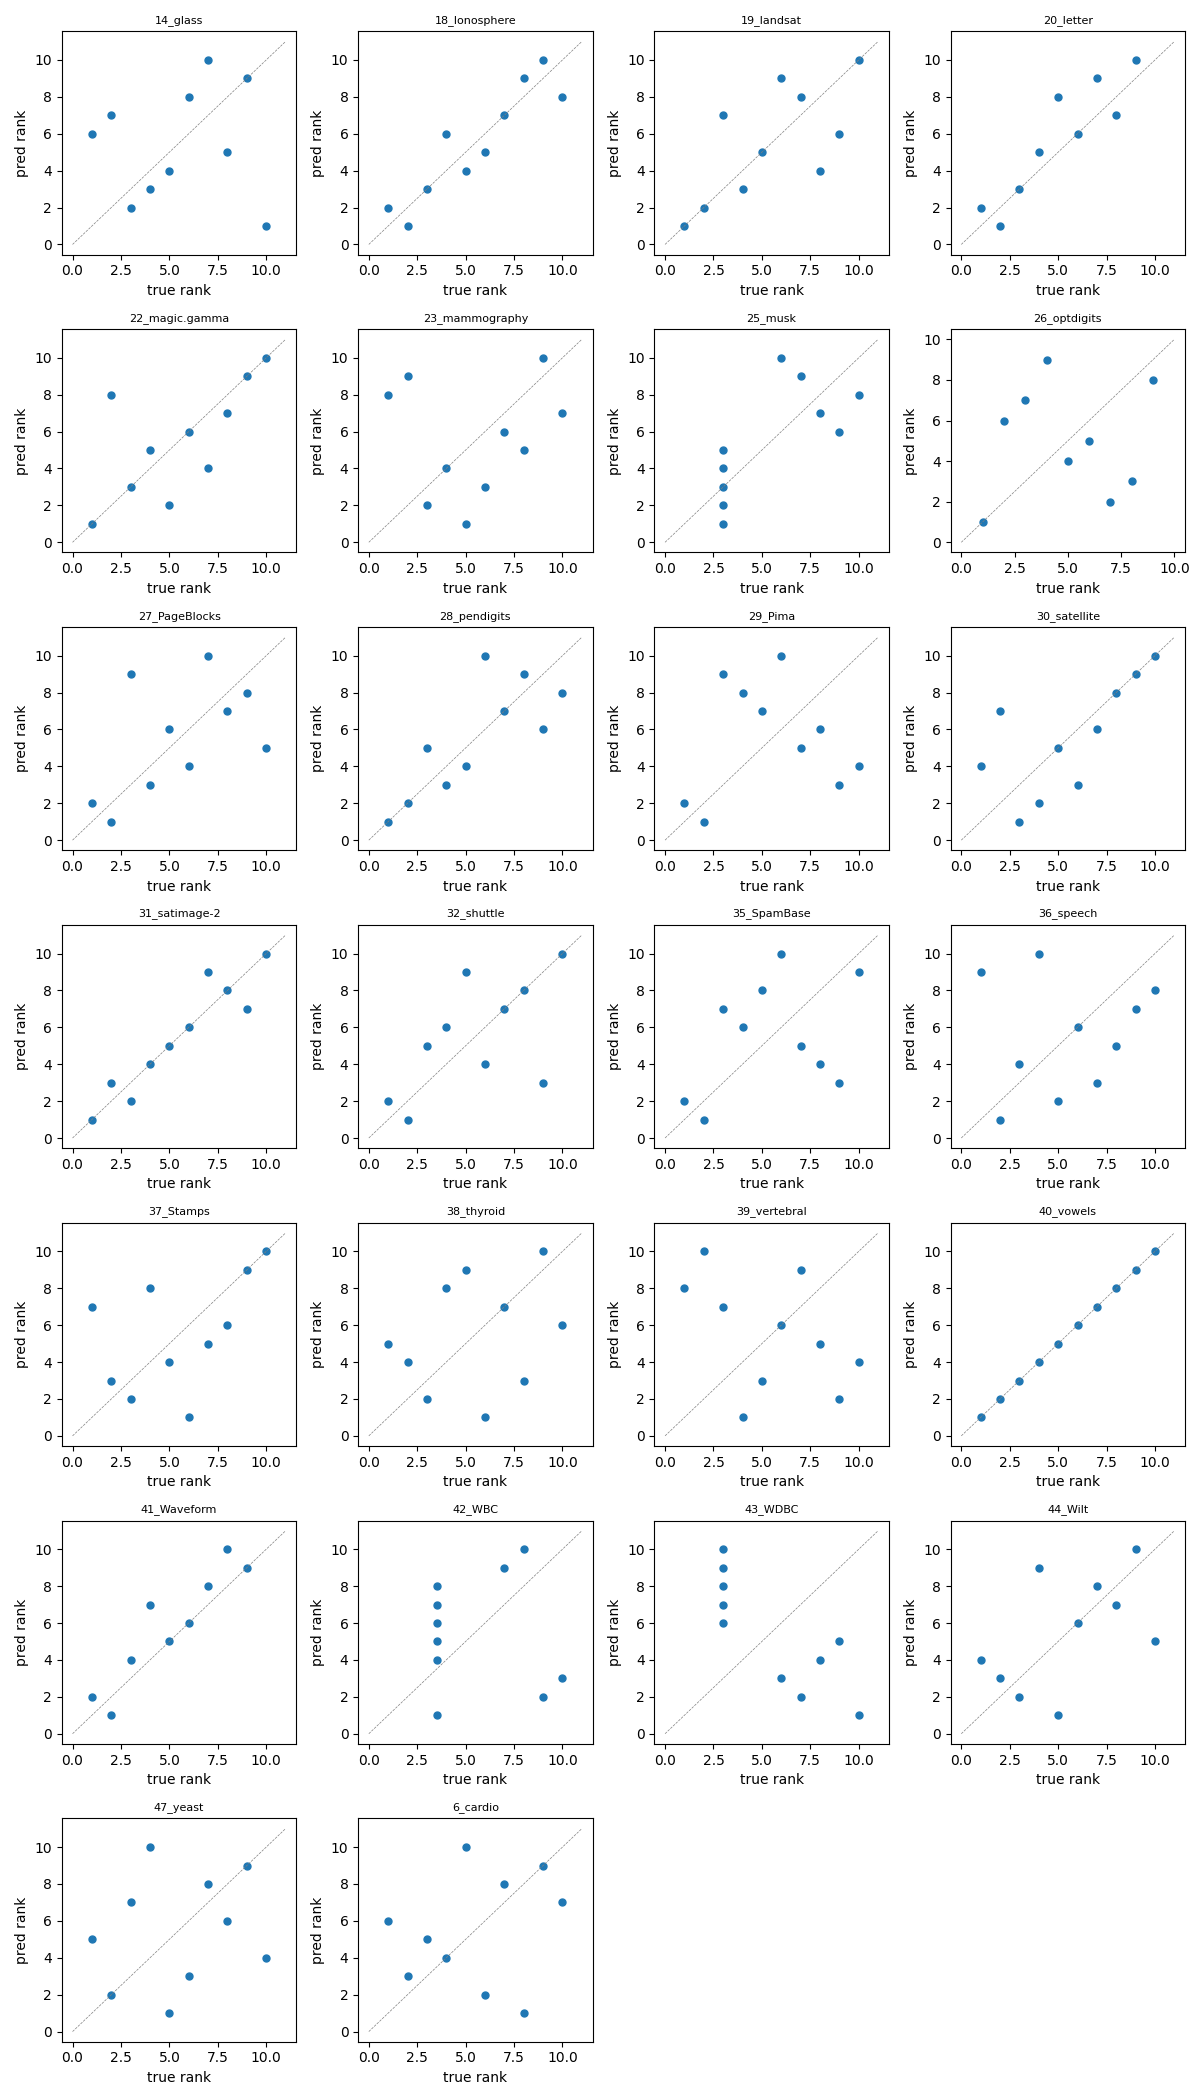
\includegraphics[width=\linewidth]{figures/fig3_scatter.png}
\caption{\textbf{Figure A.1.} Predicted rank (NoMaS) vs true rank per detector, one panel per dataset. Dashed grey identity line. Datasets where the scatter clusters near the diagonal (vowels, magic.gamma, optdigits, satellite, Pima, PageBlocks, satimage-2, Waveform) contribute the bulk of the aggregate signal. Datasets with saturated true AUC (WBC, WDBC, mammography) show noise-dominated tie-breaking.}
\end{figure}

\section{Robustness checks}\label{appendix-b-robustness-checks}

\subsection{Leave-one-detector-out panel robustness}\label{b1-leave-one-detector-out-panel-robustness}

The drop-one analysis runs on the original 10-detector panel (the nine detectors of Section 4 plus OCSVM): we recompute NoMaS $\rho$ using only 9 of the 10 detectors, dropping each one in turn (Table B.1). Baseline $\rho$ = 0.599 on the spread $\geq$ 0.10 subset with all 10.

\begin{table}[tbp]
\centering
\small\setlength{\tabcolsep}{4pt}%
\setlength{\tabcolsep}{4pt}
\begin{tabularx}{\linewidth}{>{\hsize=0.777\hsize\raggedright\arraybackslash}X >{\hsize=1.028\hsize\raggedright\arraybackslash}X >{\hsize=1.194\hsize\raggedright\arraybackslash}X}
\toprule
Dropped & $\rho$\_\allowbreak{}spread10 & $\Delta$ vs baseline \\
\midrule
IForest & 0.557 & -0.042 \\
KNN & 0.568 & -0.031 \\
PCA & 0.582 & -0.017 \\
ECOD & 0.583 & -0.016 \\
LODA & 0.602 & +0.003 \\
LOF & 0.610 & +0.011 \\
CBLOF & 0.622 & +0.023 \\
OCSVM & 0.629 & +0.030 \\
COPOD & 0.640 & +0.041 \\
HBOS & 0.642 & +0.043 \\
\bottomrule
\end{tabularx}
\end{table}

\textbf{Table B.1.} Drop-one detector robustness. $\rho$ stays in {[}0.557, 0.642{]} under any single-detector removal. Dropping the strongest single detector (IForest) is the largest loss but leaves $\rho$ well above the consensus baseline.

The ranking is stable to detector-panel choice. Dropping the strongest single detector (IForest) is the largest cost and still leaves $\rho$ = 0.557, above the consensus baseline by \textasciitilde0.7. Removing OCSVM or HBOS improves $\rho$ marginally, indicating they contribute more noise than signal to the pseudo-ranking under this panel and dataset mix; the OCSVM row is the panel-removal check referenced in Section 4.

\subsection{Deep detectors}\label{b2-deep-detectors}

\textbf{Deep detectors.} We re-run with AutoEncoder and DeepSVDD added (an 11-detector panel) on a matched spot-check (7-8 datasets per modality, single seed, K = 30 regimes) and compare against the classical 9-detector panel on the same datasets and config (Table B.2). The headline holds: auto-calibrated NoMaS still cuts regret 85-94\% below random with the deep detectors in the panel.

\begin{table}[tbp]
\centering
\small\setlength{\tabcolsep}{4pt}%
\setlength{\tabcolsep}{4pt}
\begin{tabularx}{\linewidth}{>{\hsize=0.840\hsize\raggedright\arraybackslash}X >{\hsize=1.328\hsize\raggedright\arraybackslash}X >{\hsize=1.255\hsize\raggedright\arraybackslash}X >{\hsize=0.577\hsize\raggedright\arraybackslash}X}
\toprule
Modality & 9 detectors (classical) & 11 detectors (+ deep) & Random \\
\midrule
Tabular & 0.009 (-92\%) & 0.015 (-87\%) & 0.117 \\
Image (CV) & 0.005 (-94\%) & 0.012 (-85\%) & 0.079 \\
Text (NLP) & 0.003 (-97\%) & 0.005 (-94\%) & 0.084 \\
Time-series & 0.002 (-90\%) & 0.002 (-88\%) & 0.019 \\
\bottomrule
\end{tabularx}
\end{table}

\textbf{Table B.2.} regret@1 (absolute, in AUC points; parenthetical is the reduction versus random) on the same datasets and config, classical vs deep-augmented panel, single seed. Adding two deep detectors leaves the reduction at 85-94\%. The small absolute rise (e.g. 0.009 to 0.015 on tabular) reflects a harder ranking problem, not a failure: there are two more detectors to rank and they are competitive, taking the true-best slot on three datasets (AutoEncoder once, DeepSVDD twice), so a near-miss between strong detectors costs a little regret while remaining far below random.

NoMaS v1 $\cdot$ Anomaly Detector Model Selection by Normal Manifold Separability

\end{document}
